\documentclass{article}

\usepackage{lmodern}
\usepackage[T1]{fontenc}
\usepackage[nosetpagesize]{graphicx}
\usepackage{mathpunctspace}

\title{Control the Space After Punctuation in Expressions}
\author{Yuwsuke Kieda}
\date{2018/02/27 v1.1}

\begin{document}
\maketitle

\section{Descriptions}

We provide a mechanism to control the space after the comma in the expressions.

\section{Usage}

\subsection{Sample of Preamble}

\begin{verbatim}
\usepackage{mathpunctspace}
\end{verbatim}

\subsection{Options}

\begin{itemize}
 \item unit: mu or other (default: mu)
 \item comma: substitute keyword ``natural'' or skip (default: natural)
 \item semicolon: substitute keyword ``natural'' or skip (default: natural)
 \item colon: substitute keyword ``natural'' or skip (default: natural)
 \item latexorg: original behavior of LaTeX
\end{itemize}

Remark: keyword ``natural'' mean the spacing of the in-line.

\section{License}

BSD 2-Clause License

\section{Repository}

\texttt{https://github.com/yuw/texmf-mathpunctspace}

\section{Samples}


\subsection{Sources}

\begin{verbatim}
Lorem ipsum $(x, y)$, dolor sit amet.

Lorem ipsum $\{x; x \in A\}$; dolor sit amet.

Lorem ipsum $f\colon g \to h$: dolor sit amet.
\end{verbatim}

\subsection{Sample of Options and Results}

\begin{verbatim}
\usepackage[latexorg]{mathpunctspace}
\end{verbatim}

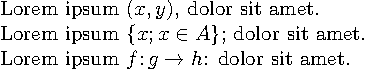
\includegraphics{latexorg.pdf}

\begin{verbatim}
\usepackage{mathpunctspace}
% same: comma=natural,semicolon=natural,colon=natural
\end{verbatim}

Lorem ipsum $(x, y)$, dolor sit amet.

Lorem ipsum $\{x; x \in A\}$; dolor sit amet.

Lorem ipsum $f\colon g \to h$: dolor sit amet.

\begin{verbatim}
\usepackage[comma=10mu,semicolon=20mu,colon=30mu]{mathpunctspace}
\end{verbatim}

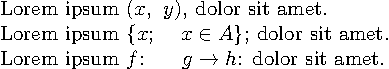
\includegraphics{comma10mu-semicolon20mu-colon30mu.pdf}

\begin{verbatim}
\usepackage[unit=pt,comma=5pt,semicolon=5pt,colon=5pt]{mathpunctspace}
\end{verbatim}

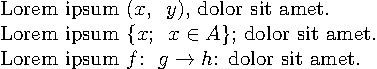
\includegraphics{comma5pt-semicolon5pt-colon5pt.pdf}

\begin{verbatim}
\usepackage[comma=0mu,semicolon=natural,colon=natural]{mathpunctspace}
\end{verbatim}

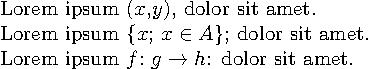
\includegraphics{comma0mu-semicolonnat-colonnat.pdf}

\section{Risks}

If the option (\texttt{comma=10mu}) is given as follows, ``right'' output can not be obtained. See \textit{The \TeX{}book} p.~134.

\begin{verbatim}
\usepackage[comma=10mu]{mathpunctspace}
\end{verbatim}

\begin{center}
 \makeatletter
 \begingroup
 \catcode`\,=\active
 \def\@x@{\def,{\thinmuskip20mu\normalcomma}}%
 \expandafter\endgroup\@x@%
% \catcode`\,=\active
% \def\@x@{\def,{\normalcomma\mskip10mu}}%
% \expandafter\endgroup\@x@%
 \makeatother
 \setbox9\hbox{,}%
 Input: \verb!$1{,}000$!\qquad
 Output: $1{,}000$\quad $1,000$
\end{center}

\end{document}
